%% LyX 2.0.3 created this file.  For more info, see http://www.lyx.org/.
%% Do not edit unless you really know what you are doing.
\documentclass[twoside,english]{paper}
\usepackage{lmodern}
\renewcommand{\ttdefault}{lmodern}
\usepackage[T1]{fontenc}
\usepackage[latin9]{inputenc}
\usepackage[a4paper]{geometry}
\geometry{verbose,tmargin=3cm,bmargin=2.5cm,lmargin=2cm,rmargin=2cm}
\usepackage{color}
\usepackage{babel}
\usepackage{float}
\usepackage{bm}
\usepackage{amsthm}
\usepackage{amsmath}
\usepackage{amssymb}
\usepackage{graphicx}
\usepackage{esint}
\usepackage[unicode=true,pdfusetitle,
 bookmarks=true,bookmarksnumbered=false,bookmarksopen=false,
 breaklinks=false,pdfborder={0 0 0},backref=false,colorlinks=false]
 {hyperref}
\usepackage{breakurl}
\usepackage{mathrsfs}

\makeatletter

%%%%%%%%%%%%%%%%%%%%%%%%%%%%%% LyX specific LaTeX commands.
%% Because html converters don't know tabularnewline
\providecommand{\tabularnewline}{\\}

%%%%%%%%%%%%%%%%%%%%%%%%%%%%%% Textclass specific LaTeX commands.
\numberwithin{equation}{section}
\numberwithin{figure}{section}

%%%%%%%%%%%%%%%%%%%%%%%%%%%%%% User specified LaTeX commands.
\usepackage{babel}

\@ifundefined{showcaptionsetup}{}{%
 \PassOptionsToPackage{caption=false}{subfig}}
\usepackage{subfig}
\makeatother

\begin{document}

\title{Notes on posterior flavour separation of fragmentation functions using SIDIS data}

%\author{Valerio Bertone, Emanuele Roberto Nocera}

%\institution{$^{a}$PH Department, TH Unit, CERN, CH-1211 Geneva 23, Switzerland}
\maketitle

%\begin{abstract}
%In this document 
%\end{abstract}
%\tableofcontents{}

%\newpage

In this set of notes we discuss a possible strategy to achieve flavour
separation of a preexisting set of fragmentation functions (FFs) using
data for semi-inclusive deep-inelastic scattering (SIDIS) with
performing a fit. The application domain of this method is the
inclusion of the COMPASS data for the production of unidentified
charged hadrons ($h^\pm$) in the set {\tt NNFF1.1h} presented in
Ref.~\cite{Bertone:2018ecm}.

\section{The methodology}

The COMPASS experiment released SIDIS data for unidentified
charged-hadrons production~\cite{COMPASS:2016xvm} in the form of
multiplicities separately for $h^+$ and $h^-$. Thanks to the partonic
structure of the corresponding observable, this data, if included in a
determination of FFs, allows one to separate, not only flavour
species, but also flavour from antiflavour. This contrasts with
single-inclusive $e^+e^-$ annihilation (SIA) data and hadro-production
in $pp$ collision that are only able to constrain a limited number of
flavour combinations. This is the reason why the NNFF1.1h set, that is
based on SIA and $pp$ data only, does not deliver a reliable flavour
separation. In these notes we device a method that allows for the
inclusion of the COMPASS data in the NNFF1.1h without the need of a
new fit. The method is based on the Bayesian reweighting procedure.

The NNFF sets adopt the following parameterisation basis:
\begin{equation}
\{D^{h^{\pm}}_{u^+},D^{h^{\pm}}_{d^++s^+},D^{h^{\pm}}_{c^+},D^{h^{\pm}}_{b^+},D^{h^{\pm}}_{g},\}
\label{eq:startingbasis}
\end{equation}
at the initial scale $Q_0=5$~GeV, with $q^+=q+\overline{q}$. This
choice, particularly the reduced number of combinations, is dictated
by the fact that the data set included in the fits is only sensitive
to this number of combinations. It is thus apparent that no separation
of $q$ and $\overline{q}$ and also of $d^+$ and $s^+$ is
achievable. This led us to parameterise the 5 combinations in
Eq.~(\ref{eq:startingbasis}) in place of the 11 independent
combinations at $Q_0$ for each hadronic charge. To obtain a separation
from SIDIS data we first assume charge conjugation symmetry to connect
the FFs of hadrons of opposite charge:
\begin{equation}
D^{h^+}_{q(\overline{q})}=D^{h^-}_{\overline{q}(q)}\,.
\label{eq:chargeconjugation}
\end{equation}
This symmetry is exact in QCD and holds at all scales. This allows us
to consider the FFs of a single charge, we choose $h^+$. Second, we
assume that ``sea-type'' quark flavours are symmetric with respect to
charge conjugation(\footnote{In fact, sice we are considering all
  possible charged hadrons in the final state, it is not strictly true
  that strange, charm, and bottom are sea-distributions. However, the
  hadronic yield is dominated by pions for which this assumption is
  more justified.}). In particular, for strange, charm, and bottom we
assume that:
\begin{equation}
D^{h^+}_q = D^{h^+}_{\overline{q}}\,,\qquad q=s,c,b\,.
\label{eq:flavoursymmetry}
\end{equation}
The 5 FF combinations in Eq.~(\ref{eq:startingbasis}) for each
hadronic charge along with the constraints in
Eqs.~(\ref{eq:chargeconjugation}) and~(\ref{eq:flavoursymmetry}),
brings us to 8 degrees of freedom constrained. To get to 11 we need
three more degrees of freedom that we constrain using the COMPASS
data. We parameterise these three additional degrees of freedom in
terms of three auxiliary functions $C(x)$, $H(x)$ and $G(x)$
introduced through the following (trivial) identities:
\begin{equation}
D^{h^+}_{u^+}(x,Q_0) = C(x) D^{h^+}_{u^+}(x,Q_0) +\left[1-C(x)\right] D^{h^+}_{u^+}(x,Q_0)\,,
\end{equation}
and identify:
\begin{equation}
D^{h^+}_{u}(x,Q_0) = C(x) D^{h^+}_{u^+}(x,Q_0)\,,\quad\mbox{and}\quad
D^{h^+}_{u}(x,Q_0)=\left[1-C(x)\right] D^{h^+}_{u^+}(x,Q_0)\,.
\label{eq:firstseparation}
\end{equation}
Then:
\begin{equation}
D^{h^+}_{d^++s^+}(x,Q_0) = H(x) D^{h^+}_{d^++s^+} (x,Q_0) +\left[1-H(x)\right] D^{h^+}_{d^++s^+} (x,Q_0)\,,
\end{equation}
and we identify:
\begin{equation}
D^{h^+}_{d^+}(x,Q_0) = H(x) D^{h^+}_{d^++s^+}(x,Q_0)
\,,\quad\mbox{and}\quad D^{h^+}_{s^+}(x,Q_0) = \left[1-H(x)\right] D^{h^+}_{d^++s^+} (x,Q_0)\,.
\end{equation}
But since we assume $D^{h^+}_{s}=D^{h^+}_{\overline{s}}$, we have that:
\begin{equation}
D^{h^+}_{s}(x,Q_0)=D^{h^+}_{\overline{s}}(x,Q_0) =
\frac12\left[1-H(x)\right] D^{h^+}_{d^++s^+} (x,Q_0)\,.
\label{eq:secondseparation}
\end{equation}
Finally, we introduce the third function as follows:
\begin{equation}
D^{h^+}_{d^+}(x,Q_0) = G(x) D^{h^+}_{d^+}(x,Q_0)+\left[1-G(x)\right]D^{h^+}_{d^+}(x,Q_0)\,,
\end{equation}
and identify:
\begin{equation}
D^{h^+}_{d}(x,Q_0) = G(x) D^{h^+}_{d^+}= G(x) H(x)
D^{h^+}_{d^++s^+}(x,Q_0)\,,
\label{eq:thirdseparation1}
\end{equation}
and:
\begin{equation}
D^{h^+}_{\overline{d}}(x,Q_0) = \left[1-G(x)\right] D^{h^+}_{d^+}=
\left[1-G(x)\right] H(x) D^{h^+}_{d^++s^+}(x,Q_0)\,.
\label{eq:thirdseparation2}
\end{equation}
At the end of the day, we can parameterise the flavour separation in
terms of $C(x)$, $H(x)$, and $G(x)$ using
Eqs.~(\ref{eq:firstseparation}),~(\ref{eq:secondseparation}),~(\ref{eq:thirdseparation1}),
and~(\ref{eq:thirdseparation2}). The final goal is the determination
of these functions. Despite, in principle, they are totally unknown, we can
in practice impose some phenomenologically-motivated constraints on them. 
First we require
that the auxiliary functions in the range $x\in [0,1]$ are between 0
and 1:
\begin{equation}
0 \leq C(x), H(x), G(x) \leq 1\,,\quad x\in [0,1]\,.
\end{equation}
The reason is that we want that the flavour-separated distributions
contribute constructively to their original combinations. We then
assume that for $x$ very close to one all flavour-separated
distributions contribute with the same amount to their original
combinations. This translates into:
\begin{equation}
C(1) = H(1) = G(1) = \frac12\,.
\end{equation}
To fulfill the requirements above it is convenient to define:
\begin{equation}
\begin{array}{l}
\displaystyle C(x) = \frac12c(x)+\frac12\,,\\
\\
\displaystyle H(x) = \frac12h(x)+\frac12\,,\\
\\
\displaystyle G(x) = \frac12g(x)+\frac12\,,
\end{array}
\end{equation}
with:
\begin{equation}
-1 \leq c(x), h(x), g(x) \leq 1\,,\quad x\in [0,1]\,,
\label{eq:bounds}
\end{equation}
and:
\begin{equation}
c(1) = h(1) = g(1) = 0\,.
\label{eq:endpoint}
\end{equation}

The simplest possible parameterisation for the functions $f=\{c,h,g\}$
is:
\begin{equation}
f(x) = Ax^\alpha(1-x)^\beta\,.
\label{eq:parameterisation}
\end{equation}
The constraint in Eq.~(\ref{eq:endpoint}) is implemented by requiring:
\begin{equation}
\beta > 0\,.
\label{eq:const1}
\end{equation}
In addition, for $f$ not to diverge at small values of $x$, we also
require:
\begin{equation}
\alpha\geq 0\,.
\label{eq:const2}
\end{equation}
The constraint in Eq.~(\ref{eq:bounds}) is implemented by requiring
that the function $f$ computed in its (unique) stationary point $x_0$
in the interval $[0,1]$ is bound to be in the interval $[-1,1]$. This
will finally result in a constraint on the normalisation factor
$A$. To do so, we first find the stationary point of $f$ by requiring
its derivative to be zero:
\begin{equation}
\left.\frac{df}{dx}\right|_{x=x_0} = A
x_0^{\alpha-1}(1-x_0)^{\beta-1}\left[\alpha-(\alpha+\beta) x_0\right]=
0 \quad\Rightarrow\quad x_0 = \frac{\alpha}{\alpha+\beta}\,,
\end{equation}
so that:
\begin{equation}
f(x_0) = A\left(\frac{\alpha}{\alpha+\beta}\right)^\alpha\left(\frac{\beta}{\alpha+\beta}\right)^\beta=A\frac{\alpha^\alpha\beta^\beta}{(\alpha+\beta)^{\alpha+\beta}}\,.
\end{equation}
Therefore, for $-1\leq f(x_0)<1$, one needs that:
\begin{equation}
-\frac{(\alpha+\beta)^{\alpha+\beta}}{\alpha^\alpha\beta^\beta}\leq
A\leq
\frac{(\alpha+\beta)^{\alpha+\beta}}{\alpha^\alpha\beta^\beta}\,.
\label{eq:const3}
\end{equation}
Finally, by extracting randomly the parameters $A$, $\alpha$, and
$\beta$ of the function $f$ defined in Eq.~(\ref{eq:parameterisation})
in the ranges allowed by the inequalities in
Eqs.~(\ref{eq:const1}),~(\ref{eq:const2}), and~(\ref{eq:const3}) for
each of the functions $c(x)$, $h(x)$, and $g(x)$, we can generate a
random flavour separation(\footnote{For obvious reason, we need to
  limit the values of $\alpha$ and $\beta$ also from above. We choose
  $\alpha,\beta < 2$ because this value seems to give a uniform
  distribution.}). We can then test the obtained flavour separation
against the experimental data by computing the corresponding
$\chi^2$. Having a broad set of random flavour separations would
subsequently allow to apply Bayesian reweighting (possibly followed
by unweighting) to select the flavour separations that best describe
the data. Fig.~\ref{fig:RandomFunctions} shows the behaviour of 100
random flavour-separation functions:
\begin{equation}
  F(x) = \frac12f(x)+\frac12\,,
\end{equation}
generated according to the recipe discussed above.
\begin{figure}[h]
  \begin{centering}
    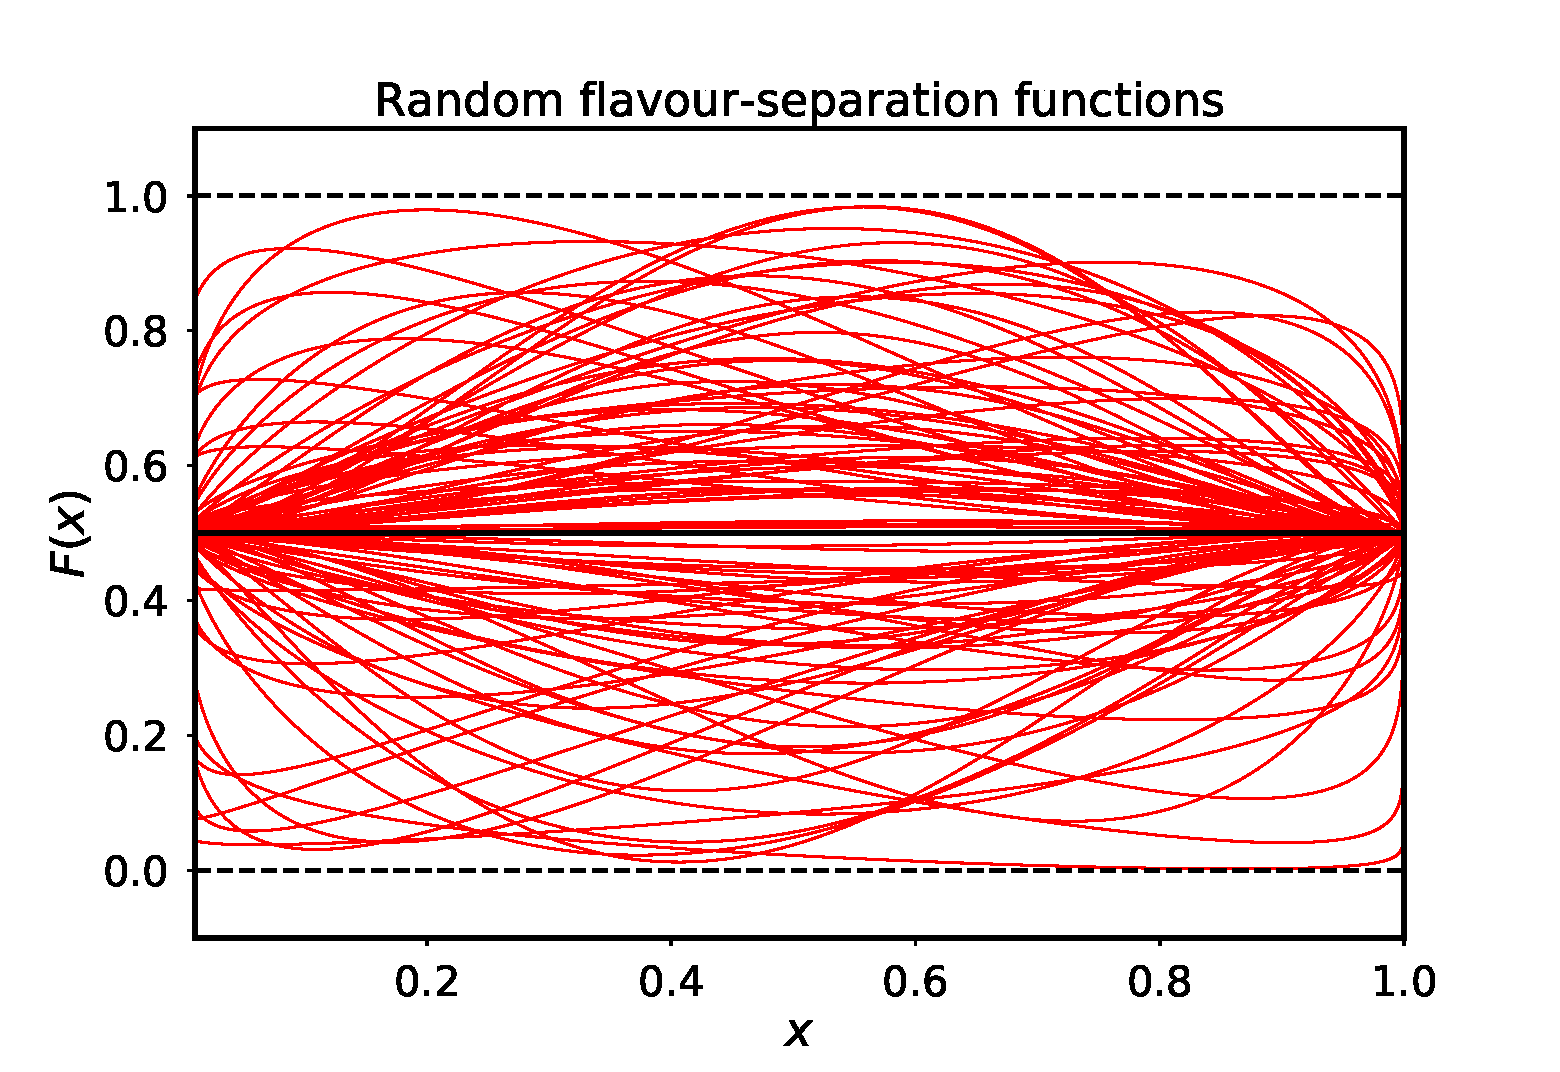
\includegraphics[width=0.8\textwidth]{plots/RandomFunctions}
    \caption{Set of 100 random flavour-separation
      functions.\label{fig:RandomFunctions}}
  \end{centering}
\end{figure}

\section{Efficient computation of the SIDIS cross section}

In this section, we will manipulate the formulas for the SIDIS cross
section so to make them optimal from the point of view of the
implementation. The goal is to make their numerical computation as
efficient as possible. The SIDIS differential cross section for the
exchange of a virtual photon can be written as:
\begin{equation}
  \frac{d^3\sigma}{dx dQdz} = 
  \frac{4\pi\alpha^2}{Q^3} 
  \left[ \frac{Y_+}{x} F_2(x,z,Q^2)
    -\frac{y^2}{x} F_L(x,z,Q^2) \right]\,,
\label{eq:sidis2}
\end{equation}
where we have defined:
\begin{equation}
Y_+ = 1+(1-y)^2\,.
\end{equation}
The structure functions $F_2$ and $F_L$ are given at NLO by the
following convolution:
\begin{equation}
\begin{array}{rcl}
  \displaystyle  F(x,z,Q) &=& \displaystyle x\sum_{q\overline{q}} e_q^2 \bigg[ 
                                    \left(C_{qq}(x,z|Q) \otimes f_q(x|Q) +   
                                    C_{qg}(x,z|Q) \otimes f_g(x|Q)\right)\otimes d_q(z|Q) \\
                                &+&\displaystyle   \left(C_{gq}(x,z|Q) \otimes f_q(x|Q)\right)\otimes d_g(z|Q) \bigg]\,,
\end{array}
\label{eq:f1sidis}
\end {equation}
where $\{f_q,f_g\}$ are the quark and gluon PDFs and $\{d_q,d_g\}$ are
the quark and gluon FFs, $e_q$ is the electric charge of the quark $q$
and $\{C^{2,L}_{qq},C^{2,L}_{qg},C^{2,L}_{gq}\}$ are the relevant
partonic cross sections. Importantly, the perturbative coefficients of
the coefficient functions $C$ factorise as follows:
\begin{equation}
C(x,z) = \sum_t c_tO_t^{(1)}(x)O_t^{(2)}(z)\,,
\label{eq:decomposition}
\end{equation}
where $c_t$ are numerical coefficients, and $O_t^{(1)}$ and
$O_t^{(2)}$ are one-dimensional functions of $x$ and $z$,
respectively. Since we are interested in isolating the FFs at some
initial scale $Q_0$, we also write:
\begin{equation}
d_{q(g)}(z|Q) = T_{q(g)i}d_{i}(z|Q) = T_{q(g)i}\Gamma_{ij}(z|Q,Q_0)\otimes d_{j}(z|Q_0)\,,
\end{equation}
where $\Gamma_{ij}$ is the appropriate evolution operator and
$T_{q(g)i}$ is the rotation matrix from the evolution to the physical
basis. Now, for the generic structure function, let us define:
\begin{equation}
\begin{array}{rcl}
\mathbb{C}_{j}(z|x,Q,Q_0) &=&\displaystyle \bigg[C_{qq}(x,z|Q) \otimes \left(\sum_{q\overline{q}}e_q^2 f_q(x|Q) T_{qi}\right) +
  \left(\sum_{q\overline{q}}e_q^2 T_{qi}\right) C_{qg}(x,z|Q) \otimes f_g(x|Q) \\
\\
&+&\displaystyle C_{gq}(x,z|Q) \otimes
    \left(\sum_{q\overline{q}}e_q^2f_q(x|Q)\right) T_{gi}\bigg]\otimes
    \Gamma_{ij}(z|Q,Q_0)\\
\\
&=&\mathbb{K}_i^{\rm SIDIS}(z|x,Q)\otimes \Gamma_{ij}(z|Q,Q_0)\,,
\end{array}
\label{eq:explicit}
\end{equation}
where we have used the fact that, in the zero-mass scheme, the quark
hard cross sections do not depend on the specific quark flavour, such
that:
\begin{equation}
  \displaystyle  F(x,z,Q) = \sum_j \mathbb{C}_{j}(z|x,Q,Q_0) \otimes d_{j}(z|Q_0)\,.
\end {equation}
Using the perturbative expansion of the hard cross sections and
Eq.~(\ref{eq:decomposition}), the factor $\mathbb{K}^{\rm SIDIS}$ in
Eq.~(\ref{eq:explicit}) can be written more explicitly as:
\begin{equation}
\begin{array}{rcl}
\mathbb{K}_{i}^{\rm SIDIS}(z|x,Q) &=&  \displaystyle\left(\sum_{q\overline{q}}e_q^2f_q(x|Q)T_{qi}\right)\delta(1-z)\\
  \\
  &+&\displaystyle a_s(Q) \sum_t
      c_{qq,t}\left[O_{qq,t}^{(1)}\otimes \left(\sum_{q\overline{q}}e_q^2 f_q(Q) T_{qi}\right)\right](x)O_{qq,t}^{(2)}(z)\\
  \\
                          &+&\displaystyle a_s(Q)\left(\sum_{q\overline{q}}e_q^2T_{qi}\right)\sum_t c_{qg,t}\left[ O_{qg,t}^{(1)}\otimes f_g(Q) \right](x)O_{qg,t}^{(2)}(z)\\
  \\
                          &+&\displaystyle a_s(Q) T_{gi}\sum_t c_{gq,t}\left[ O_{gq,t}^{(1)}\otimes
                              \left(\sum_{q\overline{q}}e_q^2f_q(Q)\right) \right](x)O_{gq,t}^{(2)}(z)\,,
\end{array}
\end{equation}
with:
\begin{equation}
a_s(Q)=\frac{\alpha_s(Q)}{4\pi}\,.
\end{equation}
Note that, given the evolution and physical basis, one has that
$T_{gi}=\delta_{gi}$ and $T_{qg}=0$. Finally, defining:
\begin{equation}
\mathbb{K}_{i}^{\rm SIDIS}(z|x,Q) =   \frac{4\pi\alpha^2}{Q^3} 
  \left[ \frac{Y_+}{x} \mathbb{K}_{2,i}^{\rm SIDIS} (z|x,Q)
    -\frac{y^2}{x} \mathbb{K}_{L,i}^{\rm SIDIS} (z|x,Q)\right]\,,
\end{equation}
one has:
\begin{equation}
  \frac{d^3\sigma}{dx dQdz} = \sum_j
  \mathbb{K}_{i}^{\rm SIDIS} (z|x,Q)\otimes\Gamma_{ij}(z|Q,Q_0)\otimes
  d_{j}(z|Q_0)\,.
\label{eq:sidisInt}
\end{equation}

\subsection{Integrating over the phase space}

For implementation reasons, we take as a reference for our
calculations the cross section differential in $x$, $Q$ and $z$
integrated over the final-state phase space (bins):
\begin{equation}
  \sigma = \int_{Q_{\rm min}}^{Q_{\rm max}}dQ \int_{x_{\rm
      min}}^{x_{\rm max}}dx \int_{z_{\rm min}}^{z_{\rm
      max}}dz\frac{d^3\sigma}{dx dQdz}\,,
\label{eq:idealintegral}
\end{equation}
However, sometimes the photon invariant mass $Q$ is replaced by the
inelasticity $y$ of the process defined as in terms of the
center-of-mass energy $\sqrt{s}$ as:
\begin{equation}
Q^2 = xys\,.
\end{equation}
In this case the integral over the phase space takes the form:
\begin{equation}
  \sigma = \int_{y_{\rm
      min}}^{y_{\rm max}}dy \int_{x_{\rm min}}^{x_{\rm max}}dx\int_{z_{\rm min}}^{z_{\rm
      max}}dz\frac{d^3\sigma}{dx dy dz}=\int_{\sqrt{x_{\rm min}y_{\rm min}s}}^{\sqrt{x_{\rm max}y_{\rm max}s}}dQ\int_{\overline{x}_{\rm min}}^{\overline{x}_{\rm
      max}}dx \int_{z_{\rm
      min}}^{z_{\rm max}}dz\frac{d^3\sigma}{dx dQ dz}\,,
\label{eq:lessidealintegral}
\end{equation}
with:
\begin{equation}
\overline{x}_{\rm min} = {\rm max}\left[x_{\rm min},\frac{Q^2}{sy_{\rm
    max}}\right]\quad\mbox{and}\quad \overline{x}_{\rm max} = {\rm min}\left[x_{\rm max},\frac{Q^2}{sy_{\rm
    min}}\right]\,.
\end{equation}
Often, cross sections are measured within a fiducial region defined
as:
\begin{equation}
W=\sqrt{\frac{(1-x)Q^2}{x}} \geq W_{\rm min}\,,\quad y_{\rm min} \leq
y\leq y_{\rm max}\,,\quad Q \geq Q_{\rm min}\,.
\end{equation}
These constraints have the effect of reducing the phase space of some
bins placed at the edge of the fiducial region. The net effect is that
of replacing the $x$ integration bounds in both
Eqs.~(\ref{eq:idealintegral}) and~(\ref{eq:lessidealintegral}) with:
\begin{equation}
  x_{\rm min}\rightarrow\overline{x}_{\rm min} = {\rm max}\left[x_{\rm min},\frac{Q^2}{sy_{\rm
        max}}\right]\quad\mbox{and}\quad x_{\rm max}\rightarrow\overline{x}_{\rm max} = {\rm min}\left[x_{\rm max},\frac{Q^2}{sy_{\rm
        min}},\frac{Q^2}{Q^2+W_{\rm min}^2}\right]\,.
\end{equation}

Therefore, also the integral in Eq.~(\ref{eq:lessidealintegral}) can
be recasted in the form of Eq.~(\ref{eq:idealintegral}). Using
Eq.~(\ref{eq:sidisInt}), we finally have that:
\begin{equation}
  \sigma = \sum_j
\left[\int_{z_{\rm min}}^{z_{\rm max}}dz  \left[\int_{Q_{\rm min}}^{Q_{\rm max}}dQ \left[\int_{x_{\rm min}}^{x_{\rm max}} dx\,\mathbb{K}_{i}^{\rm SIDIS} (z|x,Q)\right]\otimes\Gamma_{ij}(z|Q,Q_0)\right]\otimes d_{j}(z|Q_0)\right]\,.
\end{equation}
This expression provides the optimal structure for the implementation
in APFEL++ in terms of integrations and convolutions. Indeed, upon
integration in $x$, one finds:
\begin{equation}
\int_{x_{\rm min}}^{x_{\rm max}} dx\,\mathbb{K}_{i}^{\rm SIDIS} (z|x,Q)=c_i(Q;x_{\rm min},x_{\rm max})\mathbb{L}_i(z)\,,
\end{equation}
so that:
\begin{equation}
\begin{array}{rcl}
  \displaystyle \int_{Q_{\rm min}}^{Q_{\rm max}}dQ \left[\int_{x_{\rm min}}^{x_{\rm
  max}}
  dx\,\mathbb{K}_{i}^{\rm SIDIS} (z|x,Q)\right]\otimes\Gamma_{ij}(z|Q,Q_0)&=&\displaystyle \int_{Q_{\rm
                                                                 min}}^{Q_{\rm max}}dQ\,c_i(Q;x_{\rm min},x_{\rm
                                                                 max})\mathbb{L}_i(z)\otimes\Gamma_{ij}(z|Q,Q_0)\\
  \\
                                                             &=&\displaystyle\int_{Q_{\rm
                                                                 min}}^{Q_{\rm max}}dQ\,\mathbb{M}_j(z|x_{\rm min},x_{\rm
                                                                 max}, Q,Q_0)\\
  \\
                                                             &=&\displaystyle \mathbb{N}_j(z|x_{\rm min},x_{\rm
                                                                 max}, Q_{\rm min},Q_{\rm
                                                                 max},Q_0)
\end{array}
\end{equation}
and finally:
\begin{equation}
  \sigma = \sum_j
\int_{z_{\rm min}}^{z_{\rm max}}dz \,\mathbb{N}_j(z|x_{\rm min},x_{\rm
                                                                 max}, Q_{\rm min},Q_{\rm
                                                                 max},Q_0)\otimes d_{j}(z|Q_0)=\sum_j
\mathbb{O}_j({z_{\rm min}},{z_{\rm max}},x_{\rm min},x_{\rm
                                                                 max}, Q_{\rm min},Q_{\rm
                                                                 max},Q_0)\,.
\end{equation}

\section{Computation of the single-inclusive $e^+e^-$ annihilation
  cross section}

From the point of view of the numerical computation, the
single-inclusive $e^+e^-$ annihilation (SIA) cross section can be
regarded as a simplified version of the SIDIS one. Specifically, for
SIA the variable $x$ is just absent and there is no integration over
the scale $Q$ because $Q=\sqrt{s}$ with $\sqrt{s}$ fixed and
determined by the collision energy of the lepton pair. In addition, in
all cases considered in our analysis, data are delivered for specific
values of the variable $z$ such that no integration over $z$ is
required. Finally, the observable is computed as:
\begin{equation}
\frac{1}{\sigma}\frac{d\sigma}{dz} = \sum_j
  \mathbb{K}_{i}^{\rm SIA} (z|Q)\otimes\Gamma_{ij}(z|Q,Q_0)\otimes d_{j}(z|Q_0)\,.
\end{equation}
This equation closely resembles Eq.~(\ref{eq:sidisInt}) but the
$\mathbb{K}_{i}^{\rm SIA}$ functions have a simpler structure and, up
to a factor $\sigma_0/\sigma$, where $\sigma_0$ is the leading-order
total cross section, are already computed by APFEL up to
$\mathcal{O}(\alpha_s^2)$.

\newpage
\bibliographystyle{ieeetr}
\bibliography{bibliography}

\end{document}
